\subsection{Project Charter}
The project charter is a key document when working on any type of project, since it states the objectives, scope, and schedule of the project. This document will be used to define what the Eye-Tracker project is, establish the structure of the project, show and explain the cost proposal for this project, and the roles and responsibilities of each member working on this project. Another task of this document is to display to the product owner and product managers, since it will compare this project to other related products and show the improvements of this project compared to the competitors.

\subsection{Product Backlog}
The product backlog will contain all the initial requirements of the Eye-Tracker project. As the project progresses, modifications to the requirements might develop. In the case, where changes to the requirements are necessary; then this document will be updated in order for the product owner, product manager, and/or future teams to be aware of the changes in the requirements and/or product. The changes to the requirements will be explained in the document, so anyone working on this project understands why the requirement has been modified. 

\subsection{Sprint Planning}
The scrum master, product owner, and every member of the scrum team are required to attend to every sprint-planning meeting. During the meeting, the team working on the project will agree to complete a set of tasks from the product backlog. Also, the team will be able to define the sprint backlog along with the estimated time for each task; depending on the task to be completed, some of the tasks might broken down to smaller tasks. Each sprint is between 2 to 4 weeks.

\subsubsection{Sprint Goal}
The sprint goal is a description of what the team working on the product is planning to complete during the sprint. This is done, so anyone outside of the project knows what the team is currently working on. During each sprint-planning meeting and as the project progresses, the sprint goal will change.

\subsubsection{Sprint Backlog}
The sprint backlog is a list of tasks that was defined by the scrum team during the sprint-planning meeting. Each tasks in the sprint backlog is chosen from the product backlog. Scrum team members are required to keep track of the amount of hours that they spent working on each task. While completing the tasks on the sprint backlog, new items might appear for future sprints.

\subsubsection{Task Breakdown}
In order to complete certain tasks of the sprint backlog, in some cases it is helpful to breakdown each task. This will help the scrum team member organize the completion of the task as well as precisely determine the estimated time that each task will take. This is similar to an algorithm known as divide and conquer, since both involve breaking down the problem until it becomes simple to solve.

\subsection{Sprint Burndown Charts}
During each sprint, the scrum team is required to have a sprint burndown chart. Inside this chart, the spreadsheet will contain the list of each task of the sprint along with the estimated time for the task, the amount of hours worked on each tasks during the 2 to 4 weeks period, the total number of hours that each member worked on each task, and the status of the sprint tasks. In order to keep track of the sprint goal progress, the sprint burndown chart will be uploaded to the Google Drive folder shared by the team working on the project, scrum master, and product owner. 

\begin{figure}[h!]
	\centering
	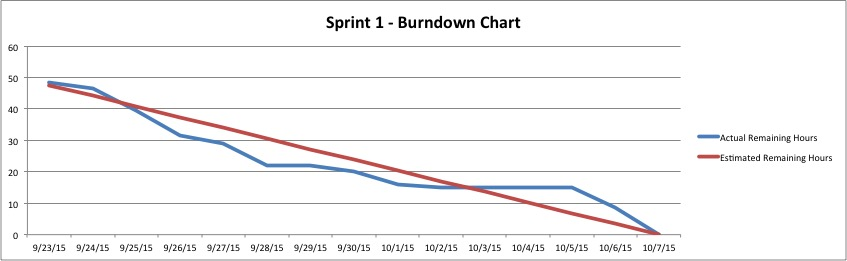
\includegraphics[width=0.90\textwidth]{images/chart}
	\caption{Sprint 1 Burndown Chart}
\end{figure}

\subsection{Sprint Retrospective}
During the sprint retrospective, the scrum master will discuss with each member of the team over the sprint session that just concluded. During this meeting, the team will also discuss what improvements can be made in order to make the future sprints more productive and successful. This meeting is very important for the project, since it may help improve the project throughout its completion. 

\subsection{Individual Status Report}
Throughout this project every member of the team is required to complete an individual status. In this report, each member will write down the task that the member has completed or is currently working on, along with the amount of hours spent on each tasks, and the future plans for the next sprint. Another item to mention in this report if while completing a task, another unexpected task appear.

\subsection{Engineering Notebooks}
Each member of the scrum team is required to obtain an engineering notebook. Inside this notebook, each member will write in detail any work performed that is related to this project. It is crucial for every member to be up to date with their entries in their engineering notebook, since it is a legal document and it is also checked periodically. 

\subsection{Closeout Materials}

\subsubsection{System Prototype}
During the life of this project, the scrum team will develop a functioning prototype of the Eye-Tracker. As the team makes progress on the project, modifications to the prototype will be performed. All the testing related to this project will be performed on this system prototype. Once the project is completed, the system prototype may be used to develop the final product. 

\subsubsection{Executive Summary}
The executive summary will give a summary of what the problem that the project is intended to solve. The purpose of this summary is for the readers to become familiar with the project without having to read all the documentation. Another purpose of this summary is to state the advantages and improvements compared to the competitors and the market that the product serves.

\subsubsection{Web Page}
The scrum team will create a static web page for advertising purpose of the product. The web page will contain pictures of the product along with the description of what the product performs, its functionality, and applications. The team will deliver the static web page in a flash drive.

\subsubsection{Demo Video}
The scrum team shall develop a video of the prototype performing its intended functions, the instructions necessary to operate the device, and an explanation of how the device performs its operations. The demo video might also be used for advertisement purpose. For better accessibility the video will be stored in a flash drive or a DVD.

\subsubsection{Source Code}
The scrum team will store the source code of the project in a Github repository for accessibility purpose while developing the product. Once the project is completed, the team will store the all the source code related to the project on a flash drive. At the moment, the product will involve programming in C++ and use the openCV library module.

\subsubsection{Source Code Documentation}
The scrum team will keep very detailed documentation in all source code related to this project. The purpose of the source code documentation is to explain how each function of the program works, so current team members or future teams that make modifications to the product do not have to expend unnecessary time attempting to understand how each function works.

\subsubsection{Hardware Schematics}
This project involves interfacing multiple hardware devices (Odroid XU4, Cypress EZ-USB CX3, and a camera module), multiple electronic components (IR LED, resistors, etc.), and a power. A schematic diagram of the product is a vital documentation that this team will provide.The schematic diagram will be stored in a flash drive as a JPEG format and in a format that the schematic diagram may be opened and altered when making modifications on future improvements.

\subsubsection{User Manual}
This scrum team will provide a user manual that will explain if any software is necessary to be installed in order to operate the product and any instructions necessary to properly operate the device. It will contain safety precautions and show pictures of how to operate the system. The documentation will be provided as PDF format and it will be stored in a flash memory.